
%(BEGIN_QUESTION)
% Copyright 2008, Tony R. Kuphaldt, released under the Creative Commons Attribution License (v 1.0)
% This means you may do almost anything with this work of mine, so long as you give me proper credit

In this 480 volt AC induction motor control circuit (sometimes referred to as a ``bucket''), a three-pole relay (typically called a {\it contactor}) is used to switch power on and off to the motor.  The contactor itself is controlled by a smaller switch, which receives 120 volts AC from a step-down transformer to energize the contactor's magnetic coil.  Although this motor control circuit used to work just fine, today the motor refuses to start.

$$\includegraphics[width=15.5cm]{i03174x01.eps}$$

Using your AC voltmeter, you measure 476 volts AC between L1 and L2, 477 volts AC between L2 and L3, and 475 volts AC between L1 and L3.  You also measure 477 volts between transformer terminals H1 and H4.  With the switch in the ``on'' position, you measure 0.5 volts AC between terminals X1 and X2 on the transformer.  From this information, identify the following:

\vskip 10pt

\begin{itemize}
\item{} \underbar{Two} components or wires in the circuit that you know cannot be failed either open or shorted, besides the 480 volt AC source which is obviously operational.
\vskip 40pt
\item{} \underbar{Two} different component or wire failures in the circuit, either one of which could account for the problem and all measured values, and the types of failures they would be (either open or shorted).
\end{itemize}

\vfil 

\underbar{file i03174}
\eject
%(END_QUESTION)





%(BEGIN_ANSWER)

This is a graded question -- no answers or hints given!

%(END_ANSWER)





%(BEGIN_NOTES)

The lack of adequate voltage at the secondary terminals of the control power transformer is a dead giveaway that something is wrong there.  We know the transformer is receiving 480 VAC (nominal) just fine, so the fault is likely within the transformer itself.

\vskip 10pt

\noindent
{\bf Components known to be in good working condition:}

\begin{itemize}
\item{} The center (L2) and right (L3) 480 VAC fuses
\item{} All wires from fuses to transformer primary
\end{itemize}

\vskip 10pt

\goodbreak
\noindent
{\bf Components which could possibly be faulted:}

\begin{itemize}
\item{} Transformer primary winding(s) failed open
\item{} Transformer secondary winding failed open
\item{} Jumper wire from H2 to H3 failed open
\end{itemize}

\vskip 10pt

Potential faults commonly listed by students, although not very likely in real life, include the following:

\begin{itemize}
\item{} Transformer secondary winding failed shorted
\item{} Contactor coil failed shorted
\end{itemize}

A shorted winding inside a transformer typically generates excessive current inside the section of winding that's been shorted, usually with spectacularly destructive results.  Smoke and fire, really!  By the same token, a shorted contactor coil would blow the fuse on the secondary side of the transformer, eliminating all load from the transformer and thus allowing the X1-X2 voltage to be its full value.

%INDEX% Troubleshooting review: electric circuits

%(END_NOTES)


